\section{Thực nghiệm và giải thích}

\subsection{Thiết lập môi trường}

\begin{itemize}
    \item \textbf{Phiên bản Python khuyến nghị:} \texttt{Python 3.8} trở lên.
    \item \textbf{Cài đặt thư viện cần thiết:}
    \begin{verbatim}
    pip install numpy networkx
    \end{verbatim}
\end{itemize}

\subsection{Hướng dẫn chạy chương trình}

\begin{itemize}
    \item \textbf{Chạy chương trình với một input và thuật toán cụ thể:}
    \begin{verbatim}
    python src/lab01.py data_file.txt <algorithm>
    \end{verbatim}
    Trong đó:
    \begin{verbatim}
    algorithms = ['bfs', 'dfs', 'ucs', 'gbfs', 'astar', 'ids', 'rbfs']
    \end{verbatim}

    \item \textbf{Ví dụ:}
    \begin{verbatim}
    python src/lab01.py data/input01.txt bfs
    \end{verbatim}

    \item \textbf{Chạy tất cả các thuật toán liên tiếp:}
    \begin{verbatim}
    python src/lab01.py data/input01.txt algorithm all
    \end{verbatim}
\end{itemize}


\subsection{Kết quả kiểm nghiệm}

\textbf{Nhắc lại:}

\begin{itemize}
    \item \textbf{BFS, DFS, IDS:} 
    Các thuật toán duyệt theo \textit{chiều rộng} và \textit{chiều sâu} đều thực hiện \textbf{Goal-test} \textit{ngay khi node con được sinh ra}, nên \textbf{Goal không thuộc tập Expanded Nodes} (các node đã mở rộng). Ngoài ra, nếu làng giềng của node được mở rộng đã có trong Frontier từ trước thì không cần thêm lại vào Frontier.
    
    \item \textbf{UCS, GBFS, A*, RBFS:} Các thuật toán sử dụng \textit{priority queue} (có hoặc không có heuristic) đều tiến hành \textbf{Goal-test} \textit{khi node được chọn để mở rộng}, 
    nhằm đảm bảo tính tối ưu hoặc hướng tìm kiếm theo heuristic. 
    Do đó, \textbf{Goal nằm trong Expanded Nodes}. Ngoài ra, nếu một node được thêm vào Frontier với chi phí nhỏ hơn thì tập tuple của node đó trước đó đã nằm trong Frontier coi như chết vì sẽ không bao giờ được duyệt đến; trong trường hợp chi phí bằng nhau thì áp dụng \textbf{tie-break rule}.

\end{itemize}

\textbf{Chú thích ký hiệu trên cây tìm kiếm:}
\begin{figure}[H]
    \centering
    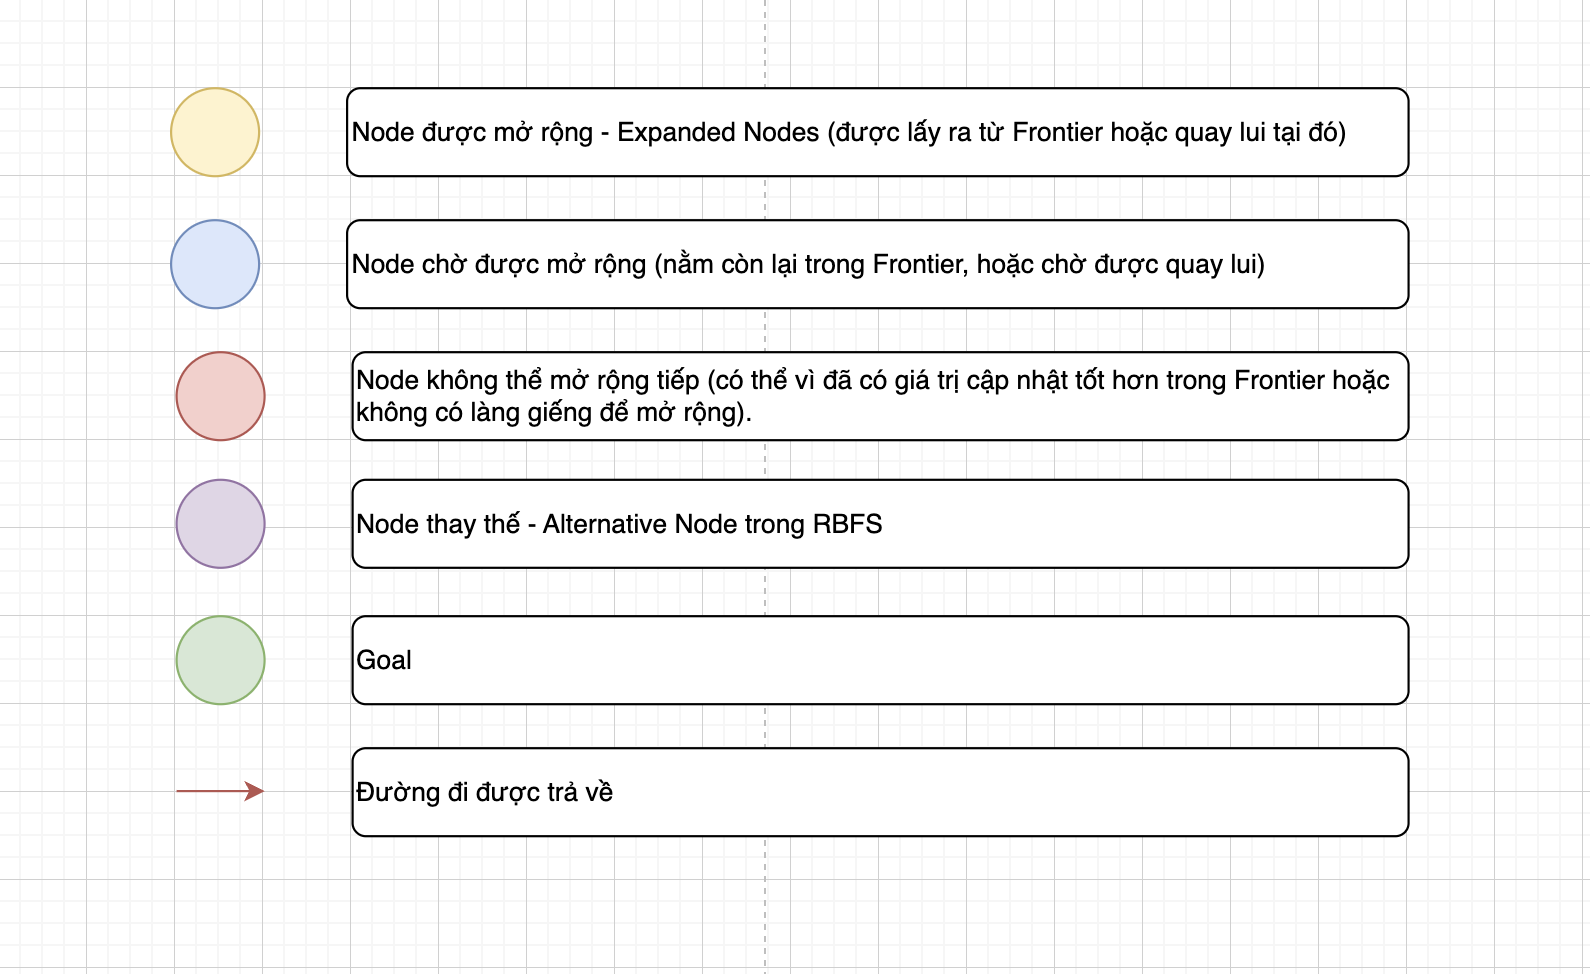
\includegraphics[scale=0.6]{img/note.png}
    \caption{Chú thích ký hiệu}
    \label{fig:my_label}
\end{figure}

\subsubsection{Input 01}

\textbf{Cấu trúc đồ thị:}

\begin{itemize}
    \item Ma trận kề gồm 8 đỉnh từ 0 đến 7:
    
    \begin{figure}[H]
    \centering
    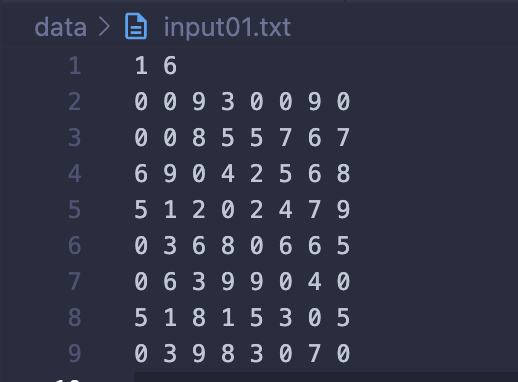
\includegraphics[scale=0.9]{img/input01.png}
    \caption{input01.txt}
    \label{fig:my_label}
    \end{figure}

    \item \textbf{Start:} 1
    \item \textbf{Goal:} 6
\end{itemize}

\textbf{Kết quả tìm kiếm:}

\begin{enumerate}

    \item \textbf{BFS:} 

    \begin{figure}[H]
        \centering
        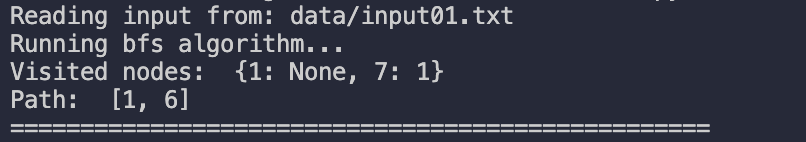
\includegraphics[scale=1.2]{img/ip1_bfs_res.png}
        \caption{Input01-BFS Result}
        \label{fig:my_label}
    \end{figure}
    
    
    \begin{figure}[H]
        \centering
        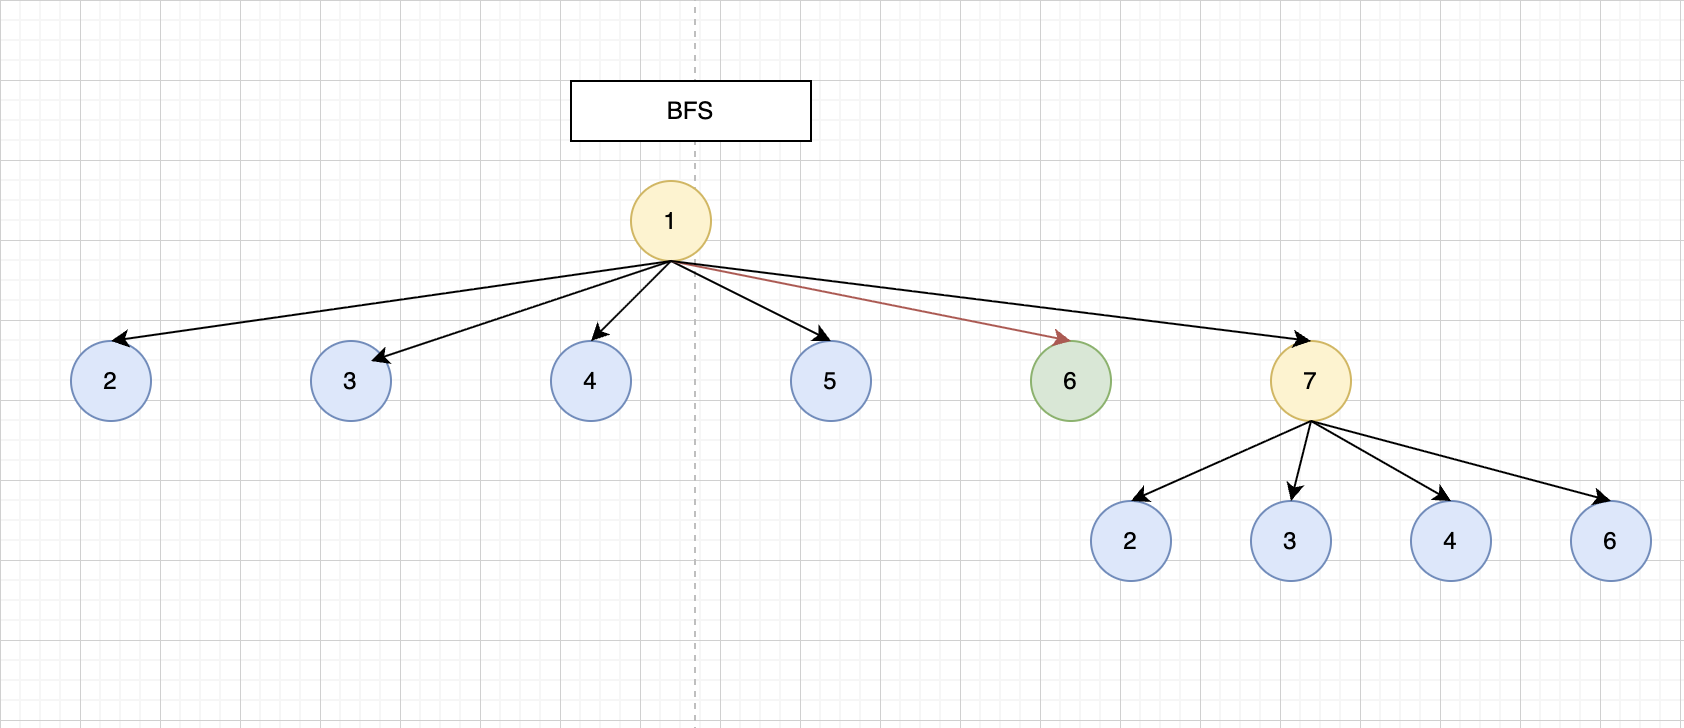
\includegraphics[scale=0.6]{img/ip1_bfs.png}
        \caption{Input01-BFS Tree Search}
        \label{fig:my_label}
    \end{figure}

    \item \textbf{UCS:}

    \begin{figure}[H]
        \centering
        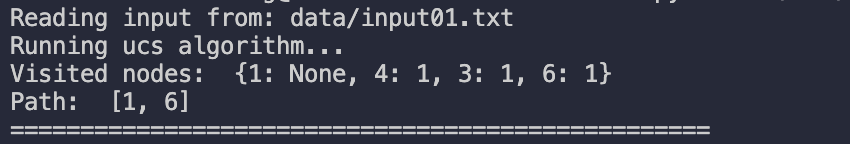
\includegraphics[scale=1.1]{img/ip1_ucs_res.png}
        \caption{Input01-UCS Result}
        \label{fig:my_label}
    \end{figure}
    
    \begin{figure}[H]
        \centering
        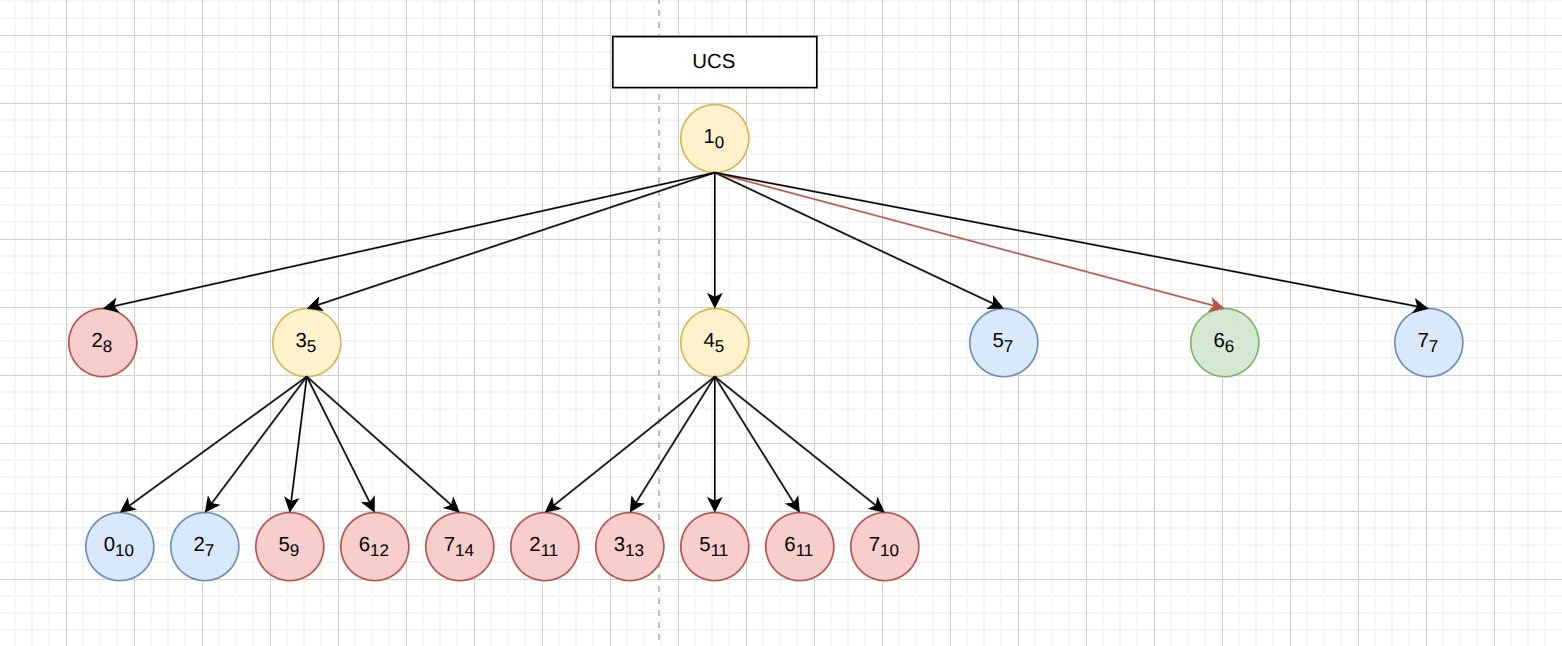
\includegraphics[scale=0.3]{img/ip1_ucs.jpg}
        \caption{Input01-UCS Tree Search}
        \label{fig:my_label}
    \end{figure} 

    \item  \textbf{DFS:}

    \begin{figure}[H]
        \centering
        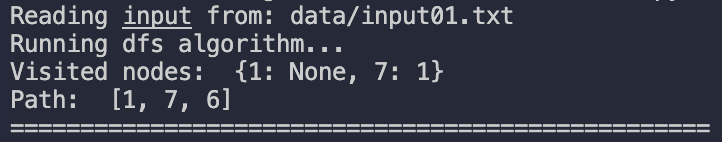
\includegraphics[scale=1.2]{img/ip1_dfs_res.png}
        \caption{Input01-DFS Result}
        \label{fig:my_label}
    \end{figure}
    
    \begin{figure}[H]
        \centering
        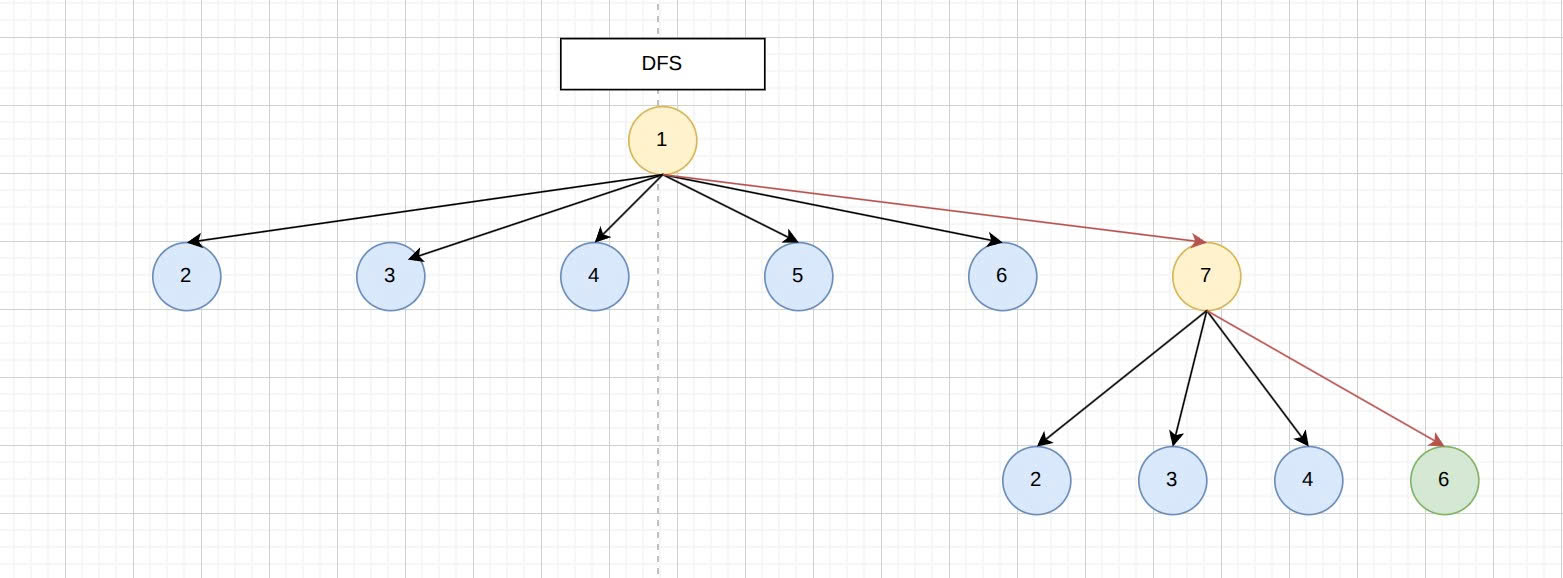
\includegraphics[scale=0.3]{img/ip1_dfs.jpg}
        \caption{Input01-DFS Tree Search}
        \label{fig:my_label}
    \end{figure}   

    
    \item  \textbf{IDS:}

    \begin{figure}[H]
        \centering
        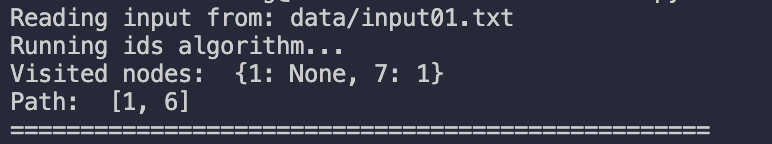
\includegraphics[scale=1.1]{img/ip1_ids_res.png}
        \caption{Input01-IDS Result}
        \label{fig:my_label}
    \end{figure}
    
    \begin{figure}[H]
        \centering
        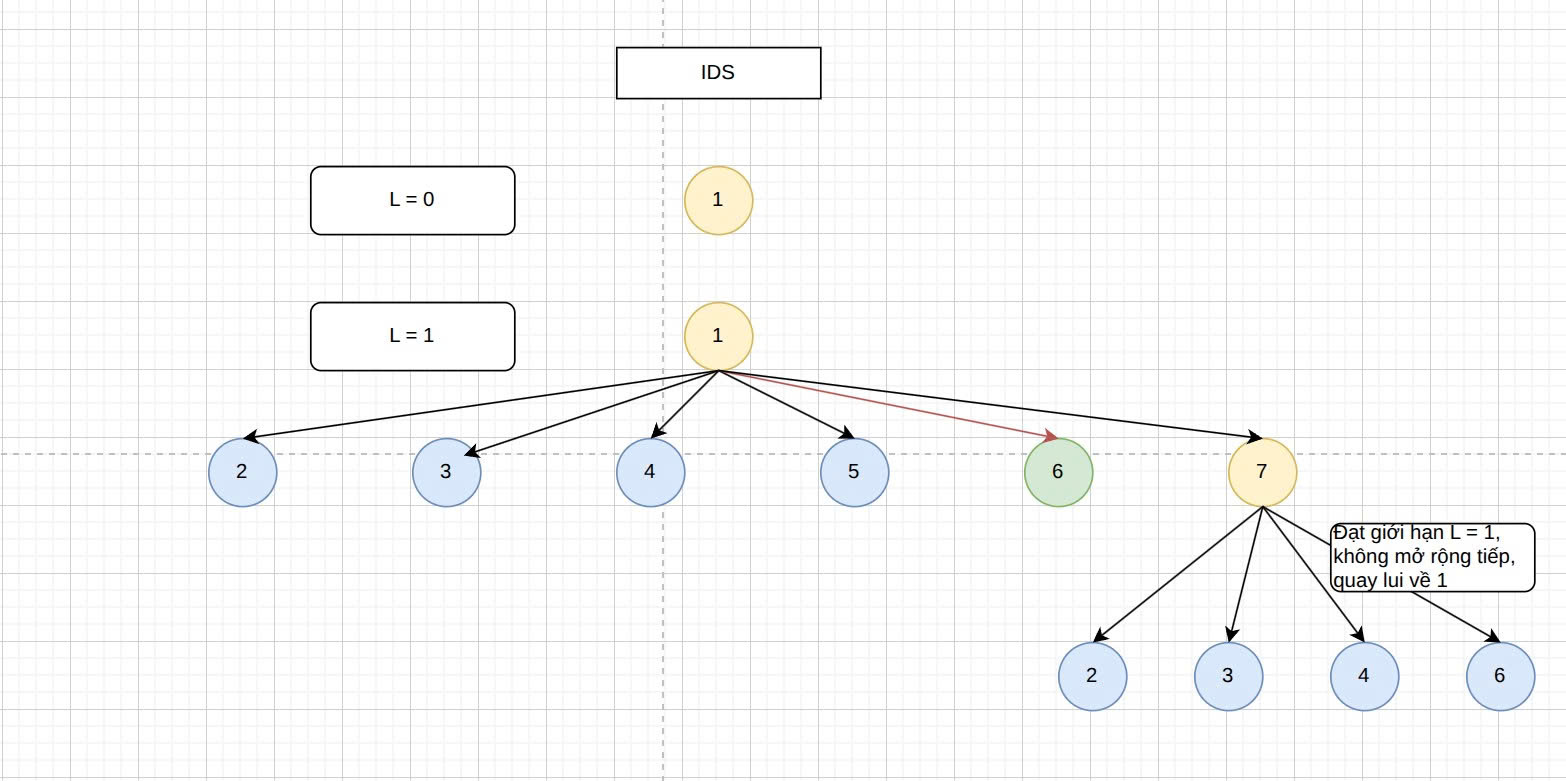
\includegraphics[scale=0.3]{img/ip1_ids.jpg}
        \caption{Input01-IDS Tree Search}
        \label{fig:my_label}
    \end{figure} 

    \item \textbf{GBFS:}

    \begin{figure}[H]
        \centering
        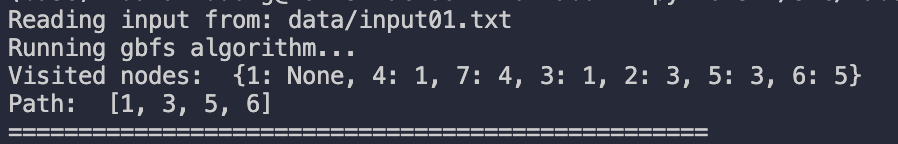
\includegraphics[scale=1]{img/ip1_gbfs_res.png}
        \caption{Input01-GBFS Result}
        \label{fig:my_label}
    \end{figure}

    \begin{figure}[H]
        \centering
        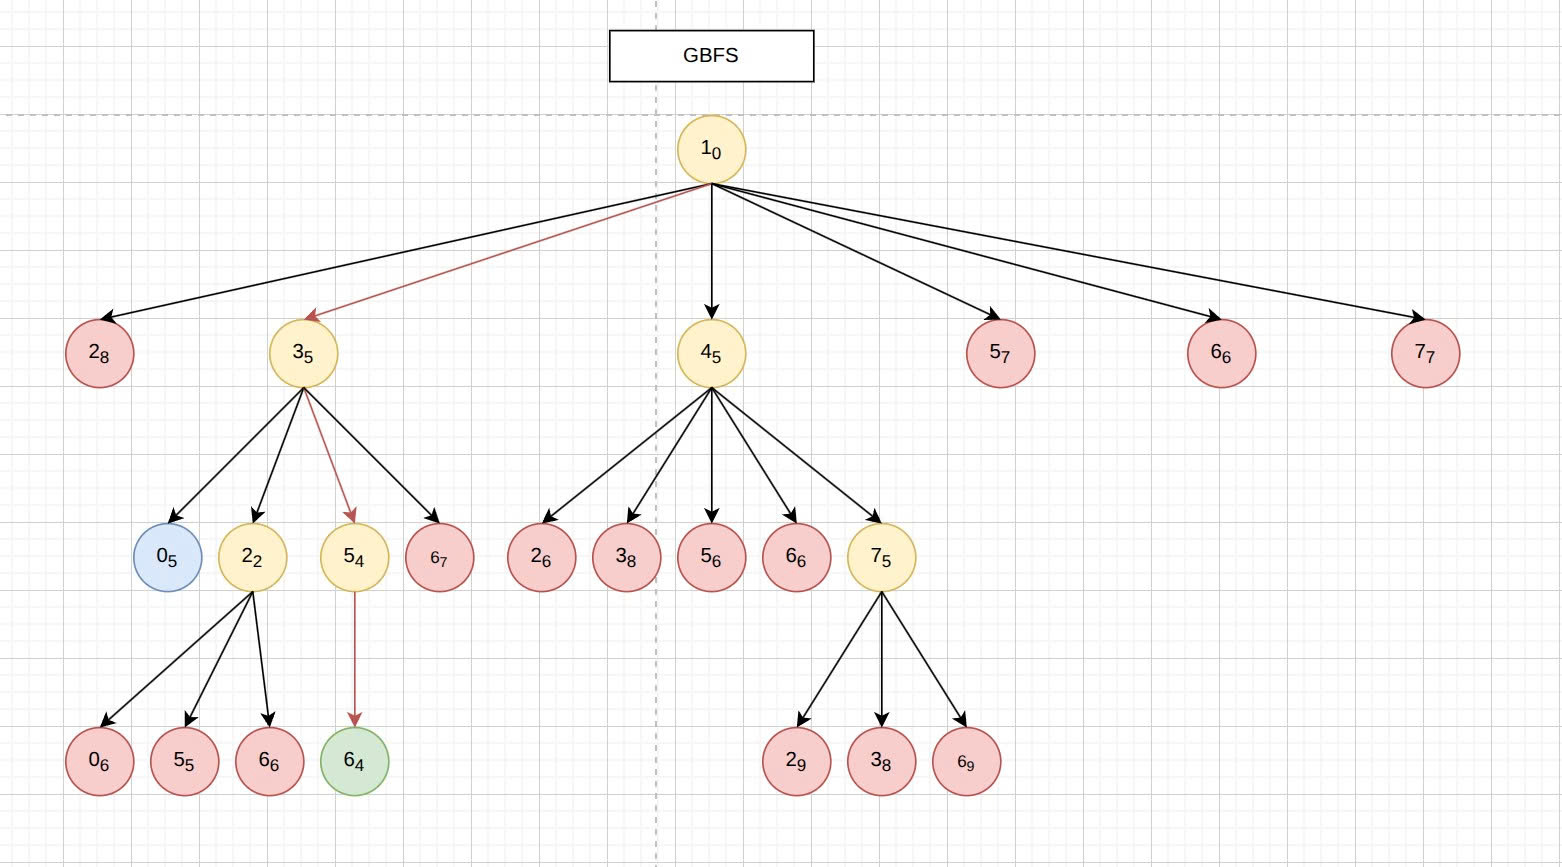
\includegraphics[scale=0.3]{img/ip1_gbfs.jpg}
        \caption{Input01-GBFS Tree Search}
        \label{fig:my_label}
    \end{figure} 

    
    \item \textbf{Astar:} 
    
    Với bảng giá trị heuristic:
    \begin{figure}[H]
        \centering
        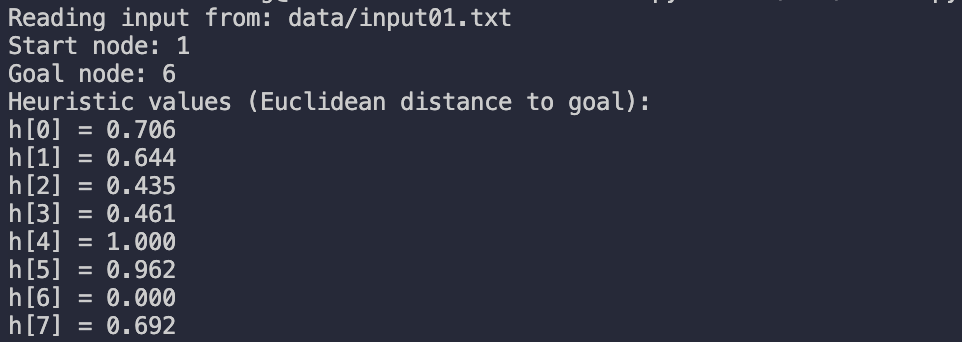
\includegraphics[scale=1]{img/ip1_heuristic.png}
        \caption{Input01-Heuristic Values}
        \label{fig:my_label}
    \end{figure}

    \begin{figure}[H]
        \centering
        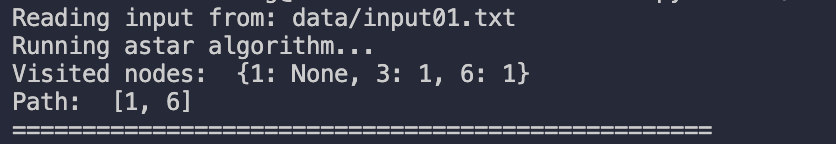
\includegraphics[scale=1.1]{img/ip1_astar_res.png}
        \caption{Input01-A* Result}
        \label{fig:my_label}
    \end{figure}

    \begin{figure}[H]
        \centering
        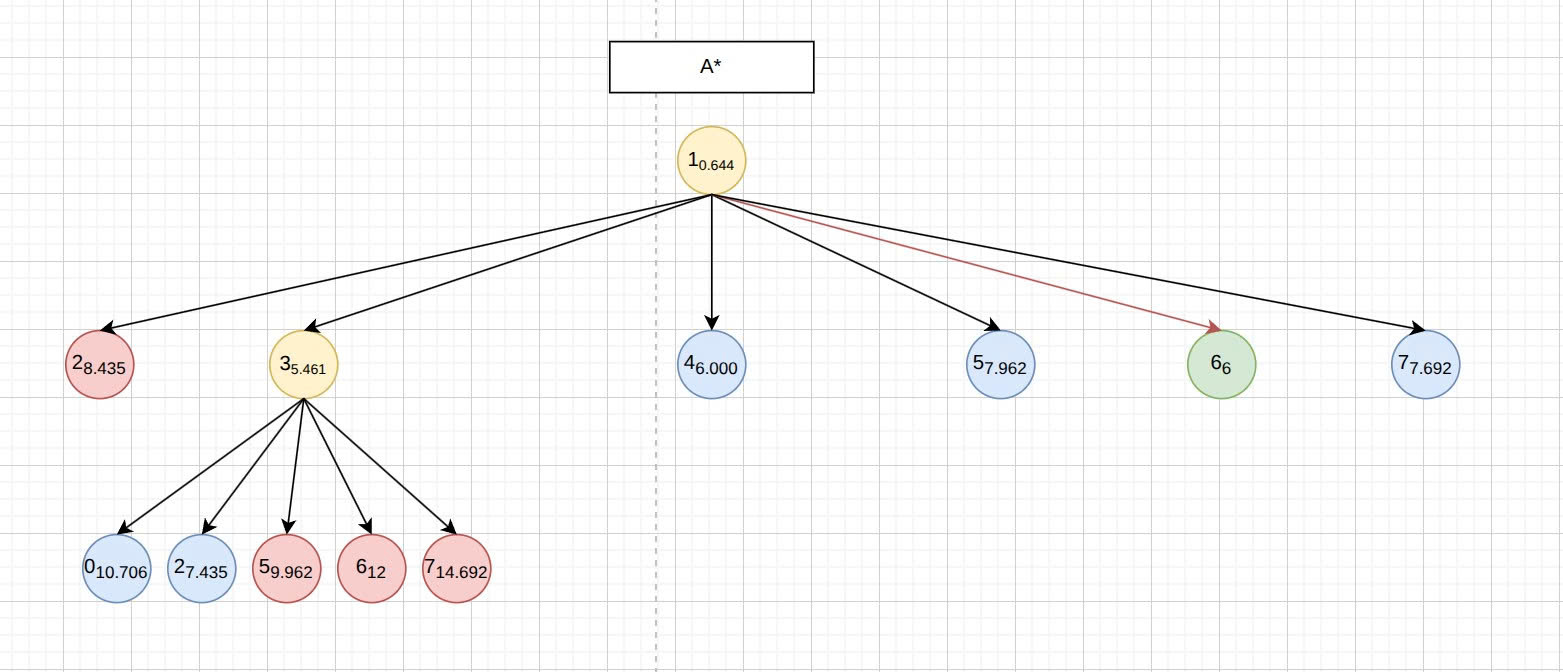
\includegraphics[scale=0.3]{img/ip1_astar.jpg}
        \caption{Input01-A* Tree Search}
        \label{fig:my_label}
    \end{figure} 

    \item \textbf{RBFS} với bảng Heuristics của Astar:

    \begin{figure}[H]
        \centering
        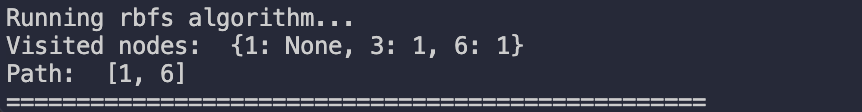
\includegraphics[scale=1.05]{img/ip1_rbfs_res.png}
        \caption{Input01-RBFS Result}
        \label{fig:my_label}
    \end{figure}
    
    \begin{figure}[H]
        \centering
        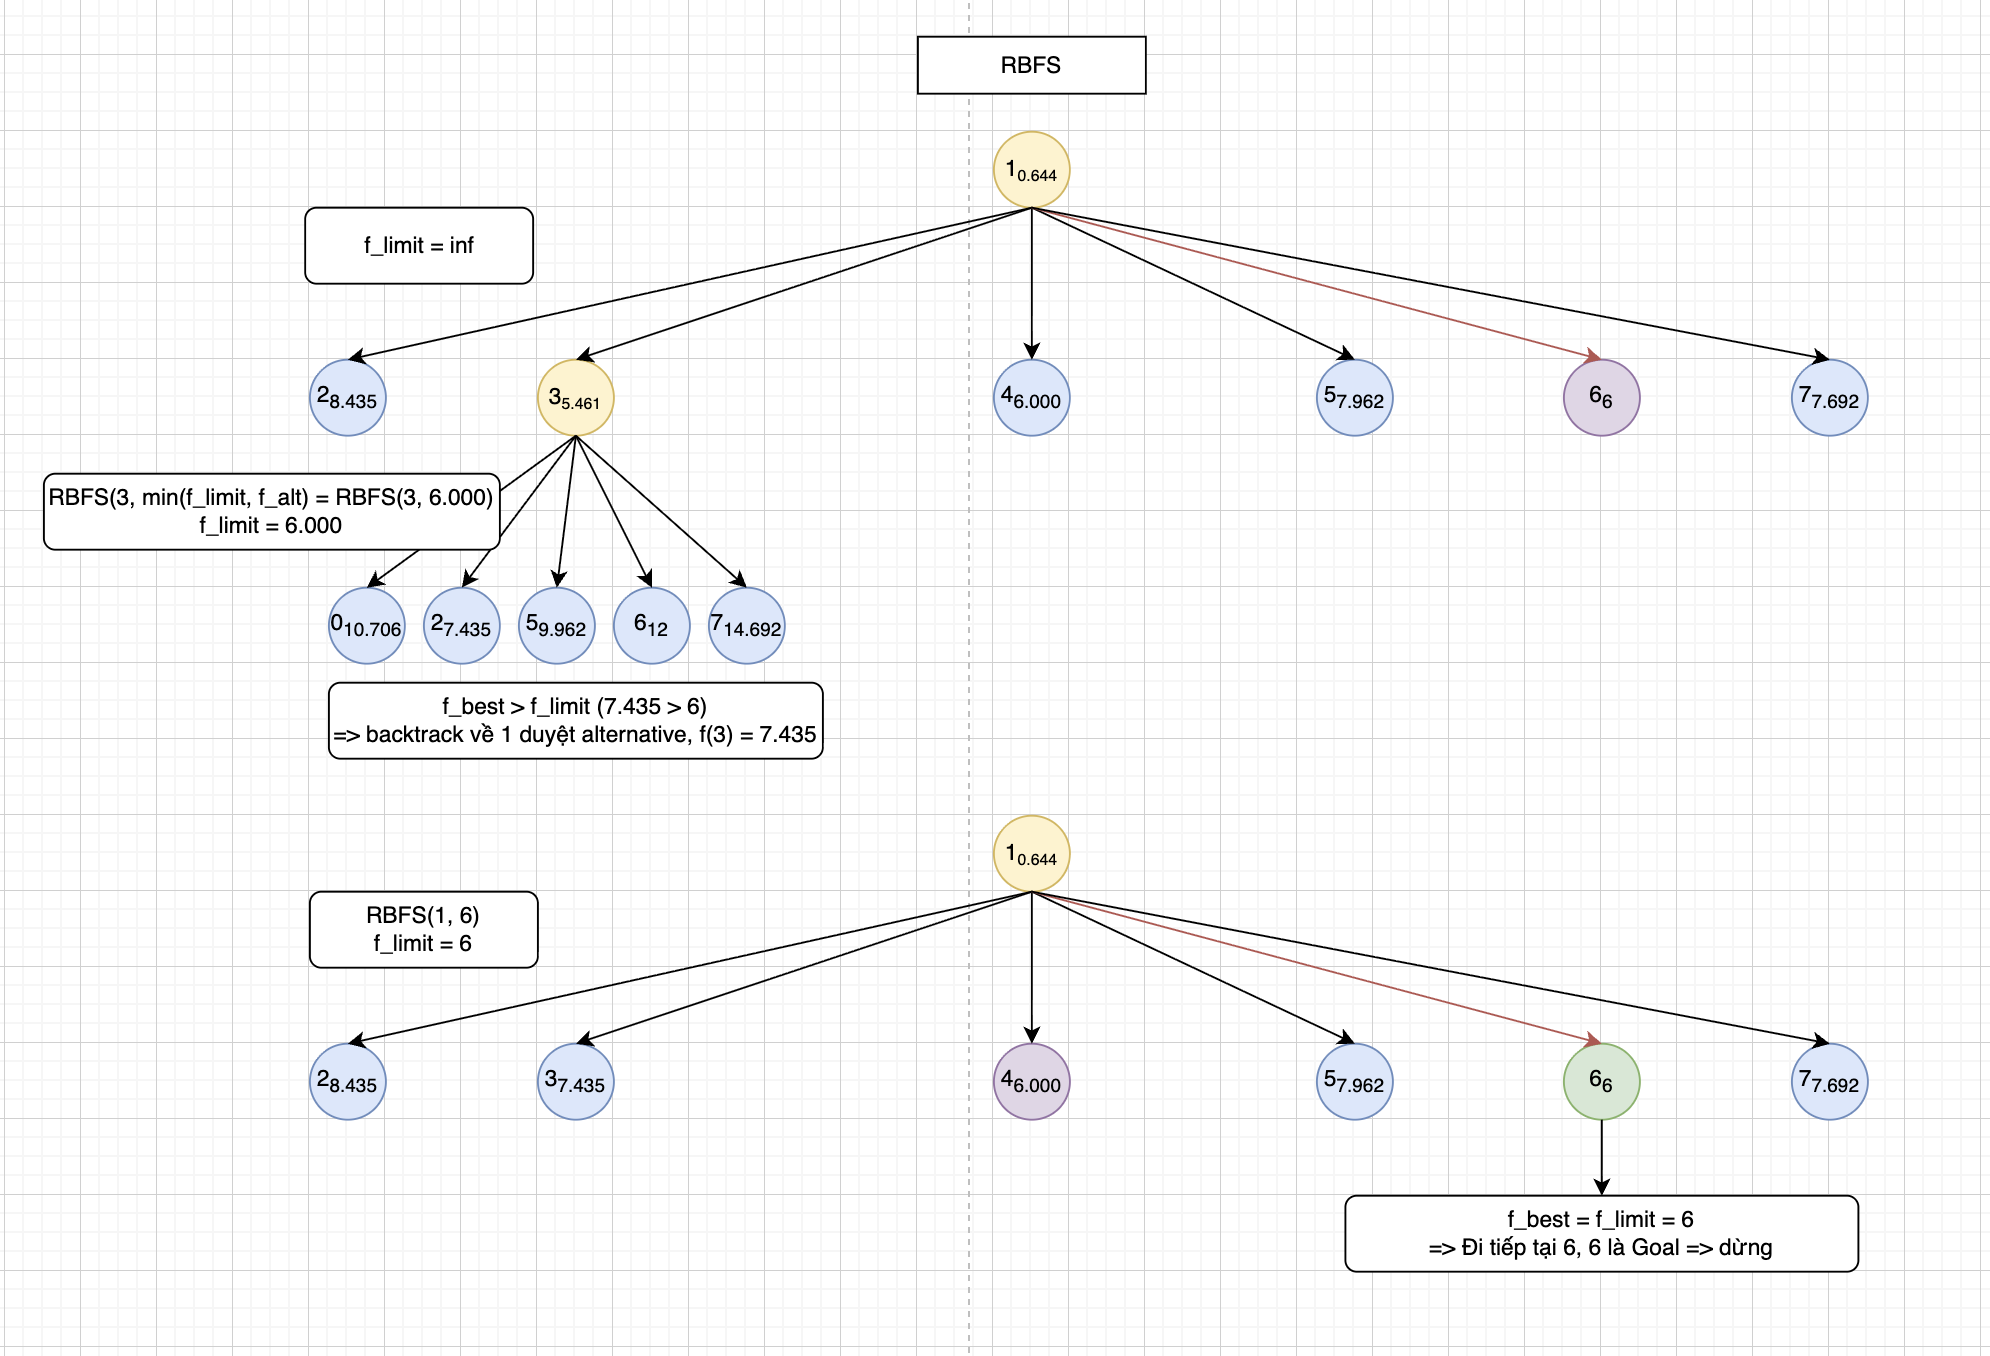
\includegraphics[scale=0.5]{img/ip1_rbfs.png}
        \caption{Input01-RBFS Tree Search}
        \label{fig:my_label}
    \end{figure} 
\end{enumerate}


\newpage

\subsubsection{Input 02}

\textbf{Cấu trúc đồ thị:}

\begin{itemize}
    \item Ma trận kề gồm 6 đỉnh từ 0 đến 5:
    
    \begin{figure}[H]
    \centering
    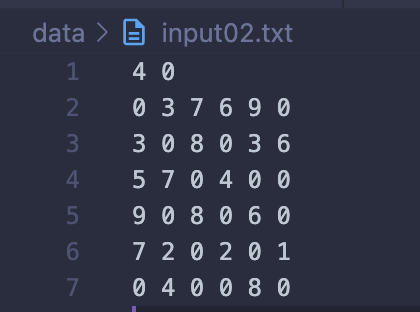
\includegraphics[scale=1]{img/input02.png}
    \caption{input02.txt}
    \label{fig:my_label}
    \end{figure}

    \item \textbf{Start:} 4
    \item \textbf{Goal:} 0
\end{itemize}

\textbf{Kết quả tìm kiếm:}

\begin{enumerate}

    \item \textbf{BFS:} 

    \begin{figure}[H]
        \centering
        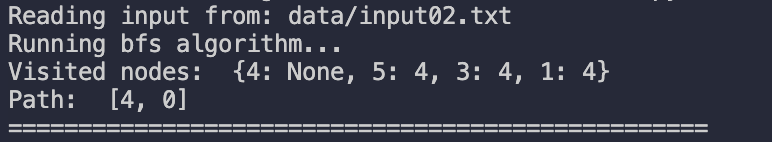
\includegraphics[scale=1.2]{img/ip2_bfs_res.png}
        \caption{Input02-BFS Result}
        \label{fig:my_label}
    \end{figure}
    
    
    \begin{figure}[H]
        \centering
        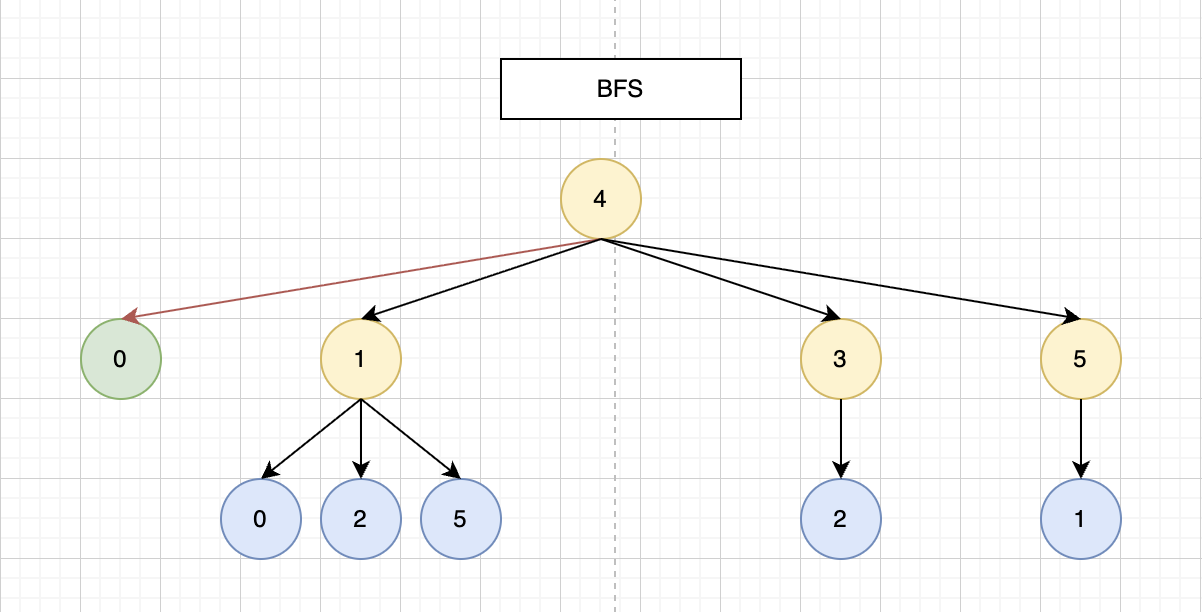
\includegraphics[scale=0.8]{img/ip2_bfs.png}
        \caption{Input02-BFS Tree Search}
        \label{fig:my_label}
    \end{figure}

    \item \textbf{UCS:}

    \begin{figure}[H]
        \centering
        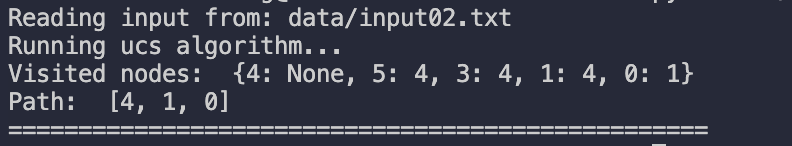
\includegraphics[scale=1.1]{img/ip2_ucs_res.png}
        \caption{Input02-UCS Result}
        \label{fig:my_label}
    \end{figure}
    
    \begin{figure}[H]
        \centering
        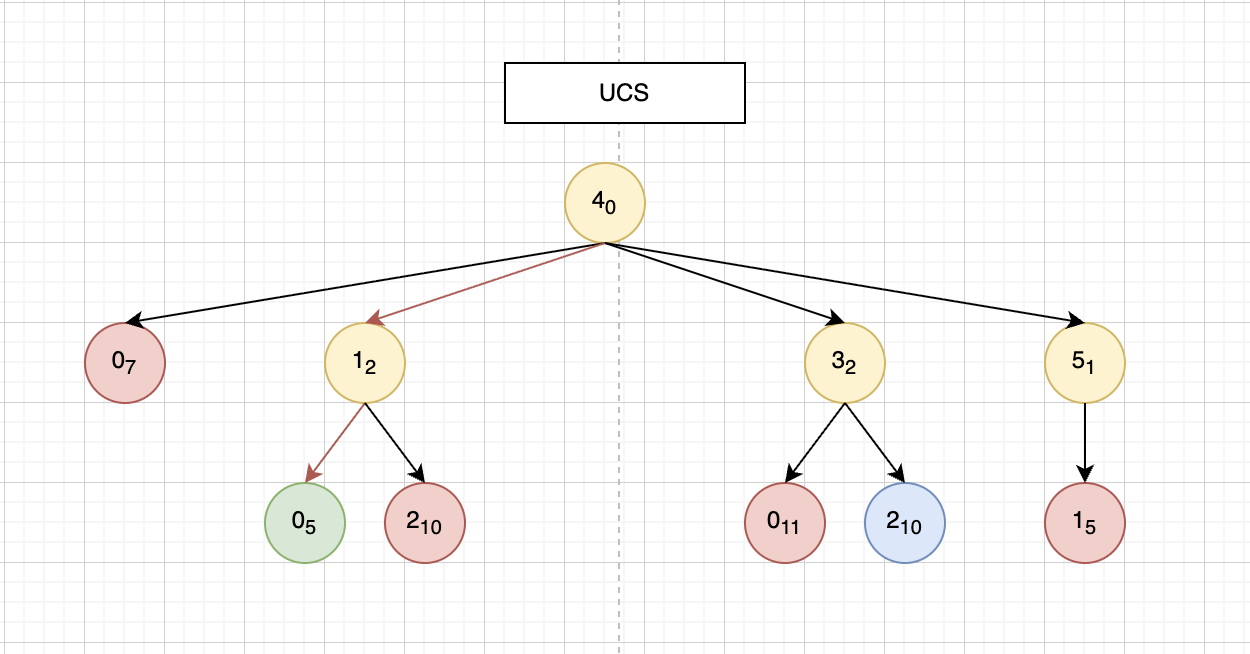
\includegraphics[scale=0.8]{img/ip2_ucs.png}
        \caption{Input02-UCS Tree Search}
        \label{fig:my_label}
    \end{figure} 

    \item  \textbf{DFS:}

    \begin{figure}[H]
        \centering
        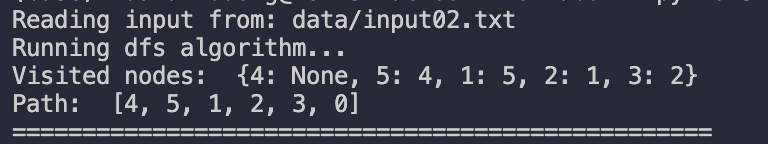
\includegraphics[scale=1.2]{img/ip2_dfs_res.png}
        \caption{Input02-DFS Result}
        \label{fig:my_label}
    \end{figure}
    
    \begin{figure}[H]
        \centering
        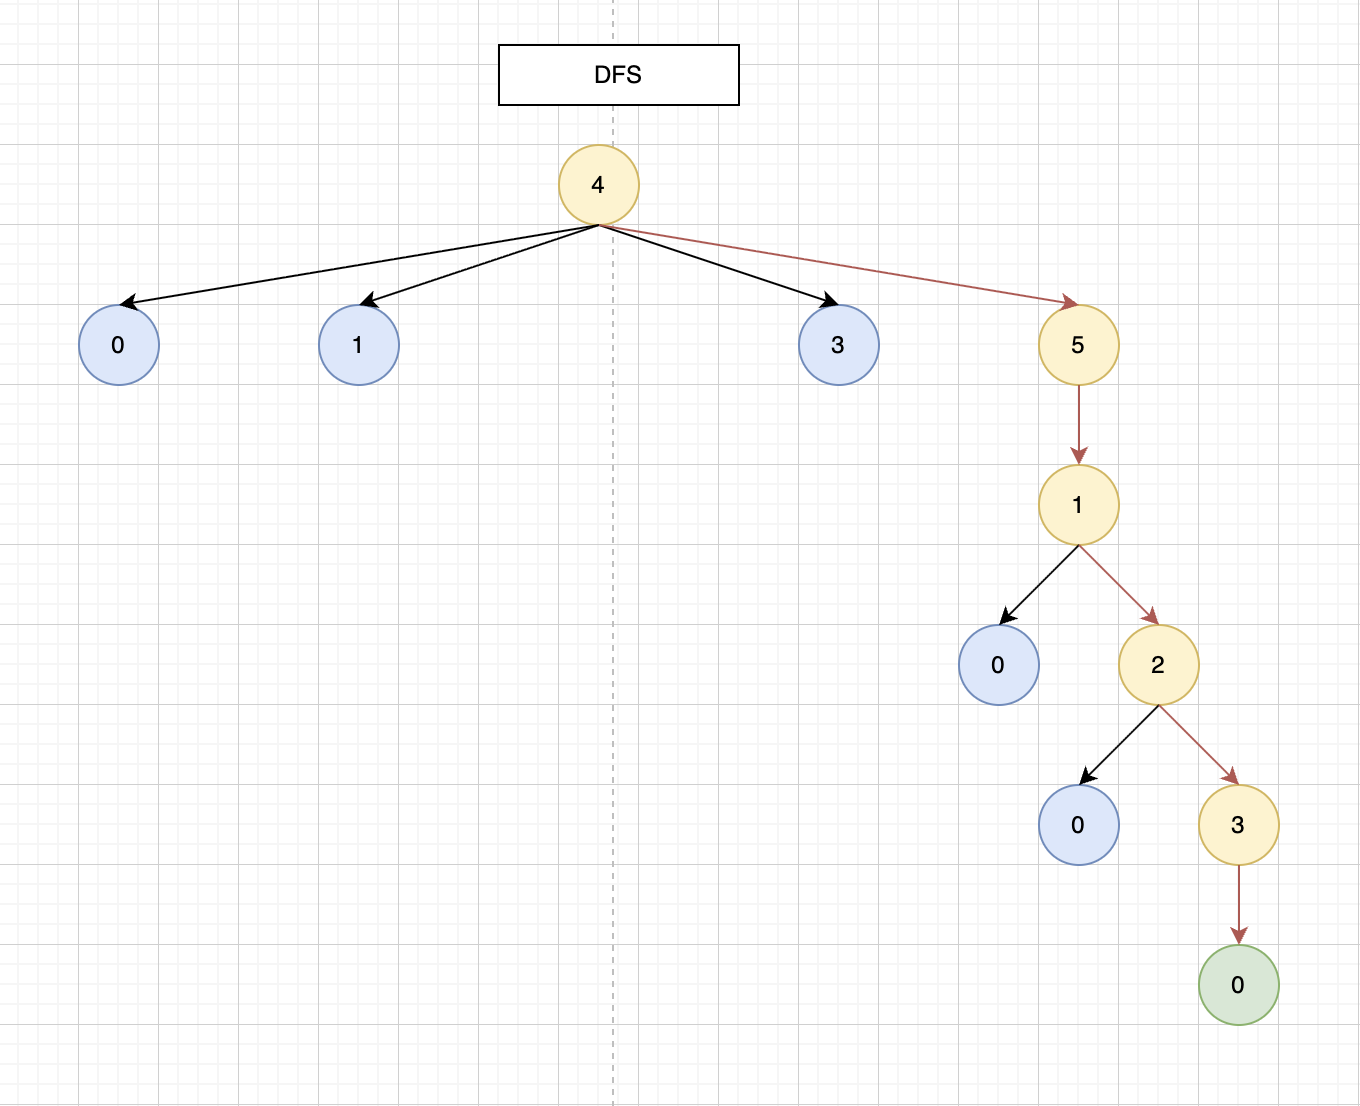
\includegraphics[scale=0.7]{img/ip2_dfs.png}
        \caption{Input02-DFS Tree Search}
        \label{fig:my_label}
    \end{figure}   

    
    \item  \textbf{IDS:}

    \begin{figure}[H]
        \centering
        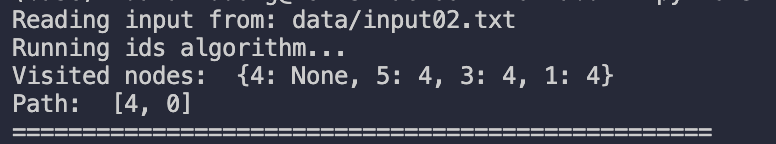
\includegraphics[scale=1.1]{img/ip2_ids_res.png}
        \caption{Input02-IDS Result}
        \label{fig:my_label}
    \end{figure}
    
    \begin{figure}[H]
        \centering
        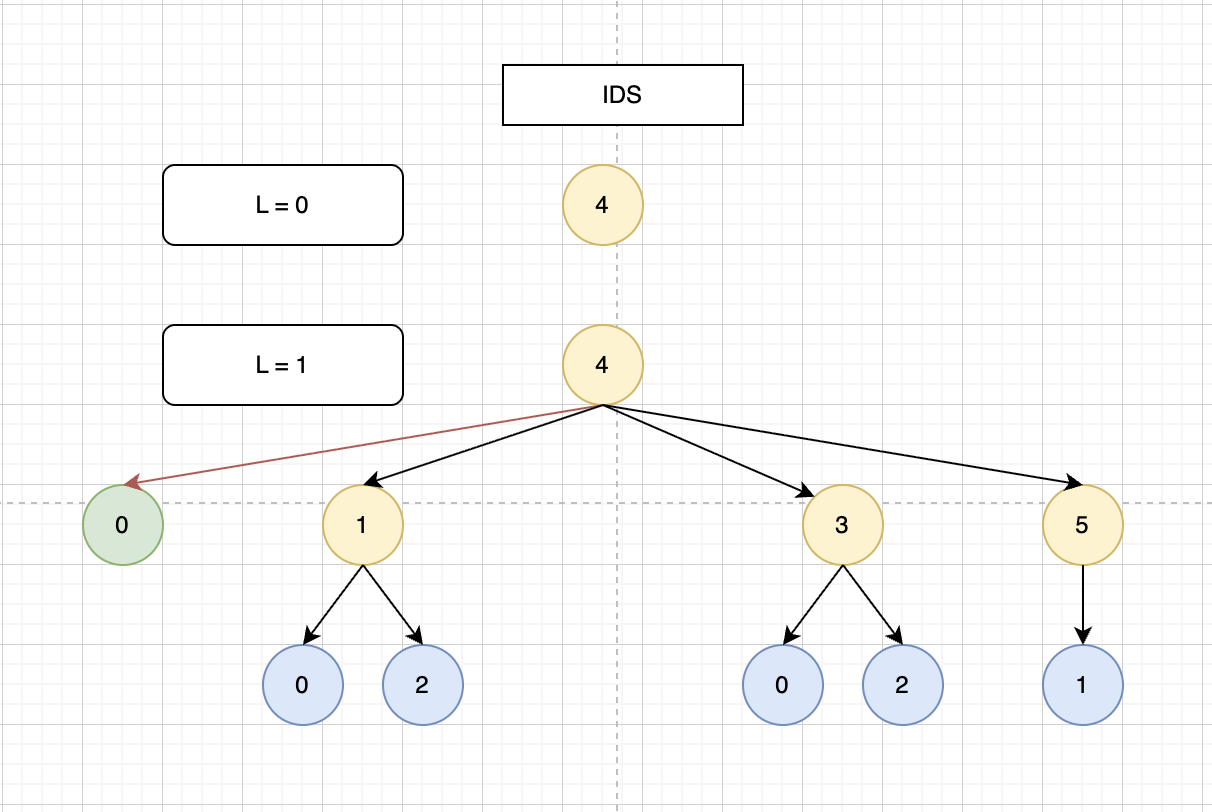
\includegraphics[scale=0.7]{img/ip2_ids.png}
        \caption{Input02-IDS Tree Search}
        \label{fig:my_label}
    \end{figure} 

    \item \textbf{GBFS:}

    \begin{figure}[H]
        \centering
        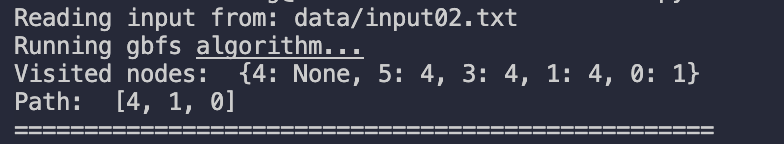
\includegraphics[scale=1]{img/ip2_gbfs_res.png}
        \caption{Input02-GBFS Result}
        \label{fig:my_label}
    \end{figure}

    \begin{figure}[H]
        \centering
        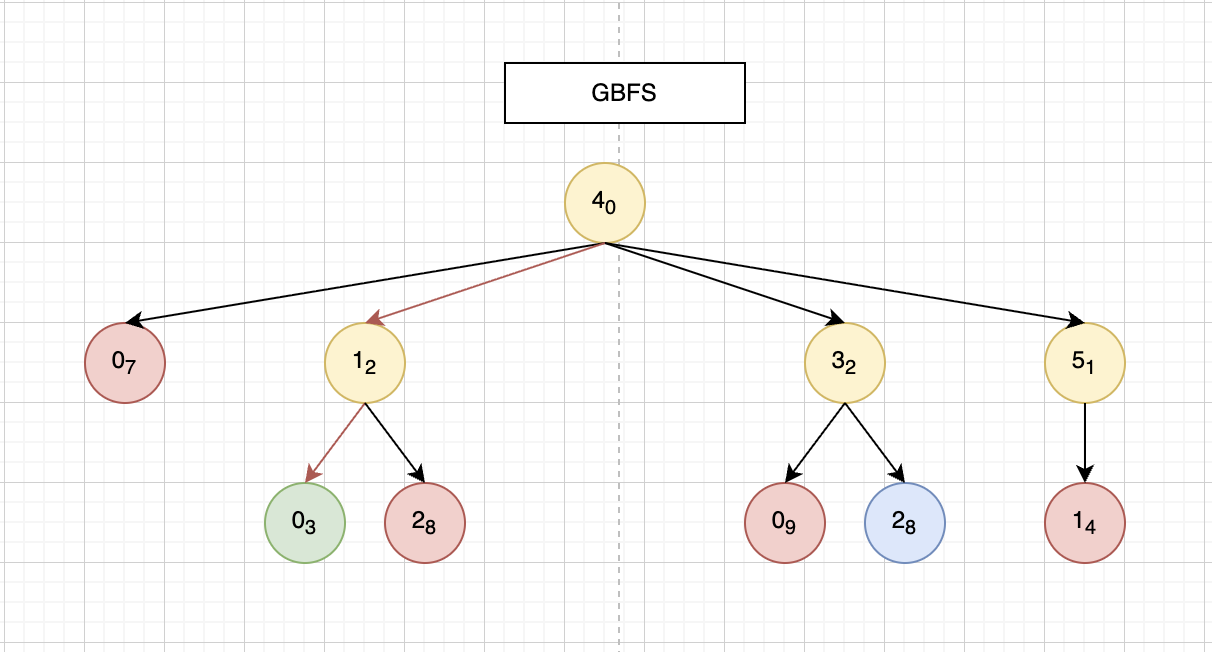
\includegraphics[scale=0.7]{img/ip2_gbfs.png}
        \caption{Input02-GBFS Tree Search}
        \label{fig:my_label}
    \end{figure} 

    
    \item \textbf{Astar:} 
    
    Với bảng giá trị heuristic:
    \begin{figure}[H]
        \centering
        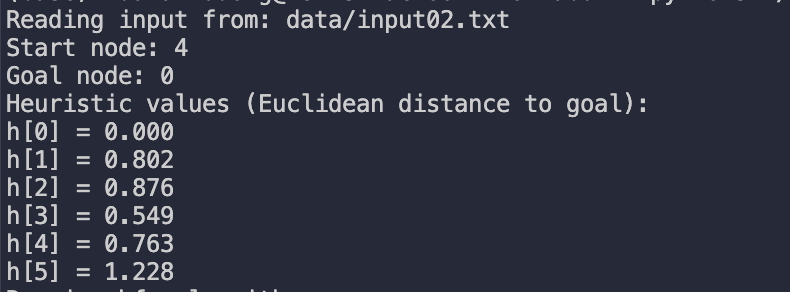
\includegraphics[scale=1]{img/ip2_heuristic.png}
        \caption{Input02-Heuristic Values}
        \label{fig:my_label}
    \end{figure}

    \begin{figure}[H]
        \centering
        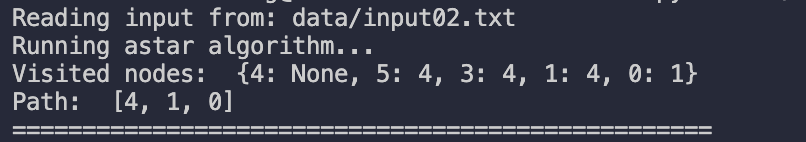
\includegraphics[scale=1.1]{img/ip2_astar_res.png}
        \caption{Input02-A* Result}
        \label{fig:my_label}
    \end{figure}

    \begin{figure}[H]
        \centering
        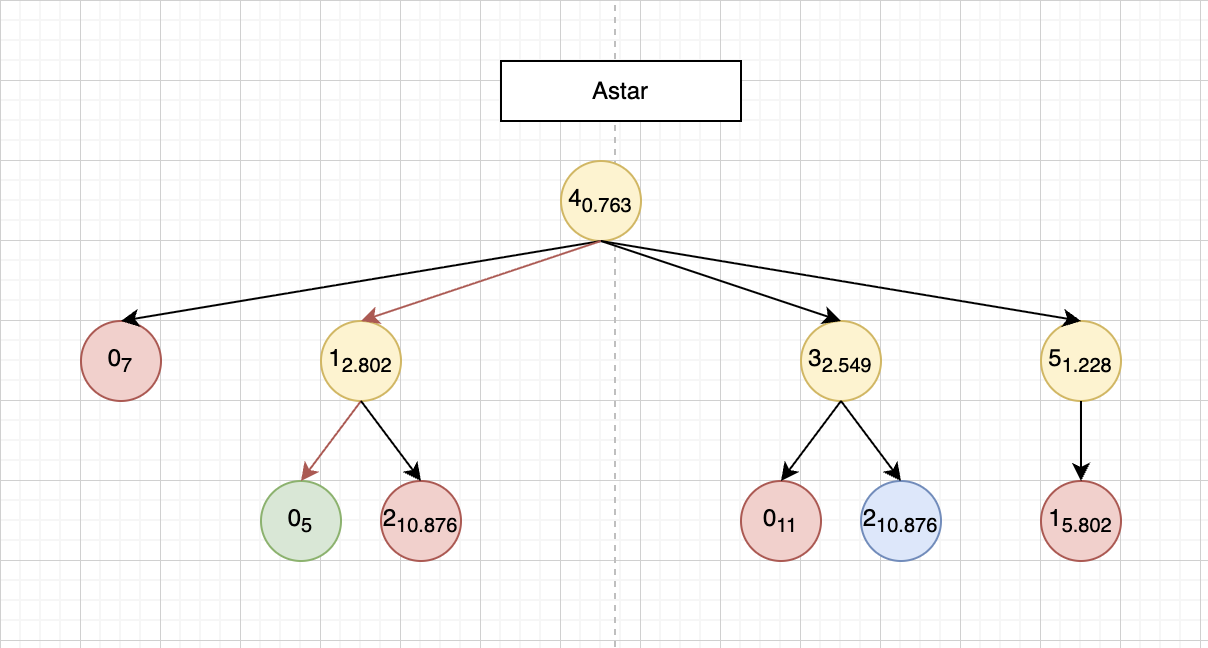
\includegraphics[scale=0.7]{img/ip2_astar.png}
        \caption{Input02-A* Tree Search}
        \label{fig:my_label}
    \end{figure} 

    \item \textbf{RBFS} với bảng Heuristics của Astar:

    \begin{figure}[H]
        \centering
        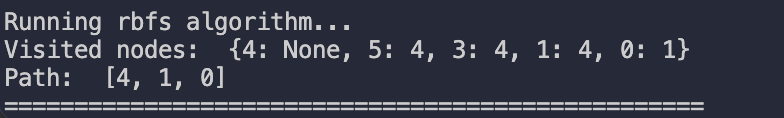
\includegraphics[scale=1.05]{img/ip2_rbfs_res.png}
        \caption{Input02-RBFS Result}
        \label{fig:my_label}
    \end{figure}
    
    \begin{figure}[H]
        \centering
        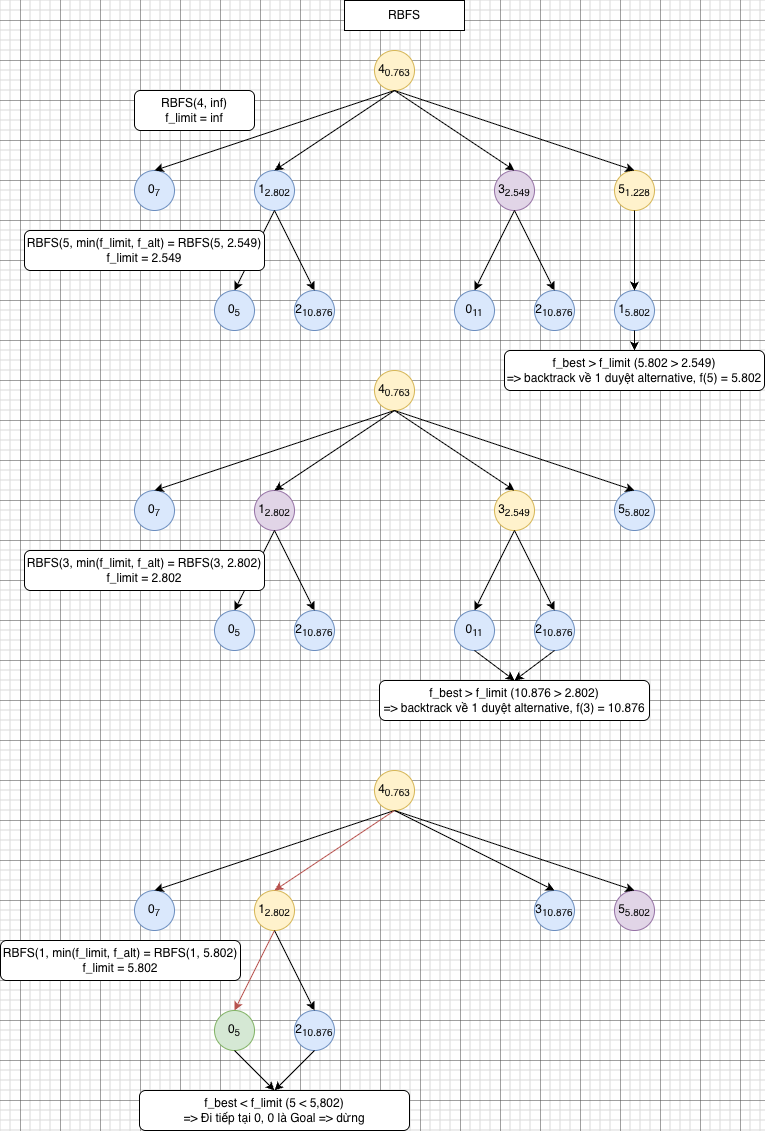
\includegraphics[scale=0.6]{img/ip2_rbfs.png}
        \caption{Input02-RBFS Tree Search}
        \label{fig:my_label}
    \end{figure} 
\end{enumerate}


